\documentclass[11pt]{article}

\usepackage[margin=1in]{geometry}
\usepackage{amssymb,amsmath}
\usepackage[final]{graphicx}
\graphicspath{ {./images/} }

\usepackage[hyphens]{url}
\usepackage{hyperref}
\hypersetup{
    colorlinks=true,
    linkcolor=blue,
    filecolor=magenta,      
    urlcolor=cyan,
    citecolor = black
} 

\usepackage{fancyhdr}
\pagestyle{fancy}
\fancyhead[L,C]{}
\fancyhead[R]{}
\fancyfoot[L]{}
    \fancyfoot[R]{\thepage}
\fancyfoot[C]{}

\usepackage{titlesec}
\titleformat{\section}[block]{\Large\bfseries\filcenter}{}{1em}{}
\titleformat{\subsection}[hang]{\bfseries}{}{1em}{}
\setcounter{secnumdepth}{0}

\begin{document} 


\section{Chapter 7}

On question 26:

\vspace{-30mm}
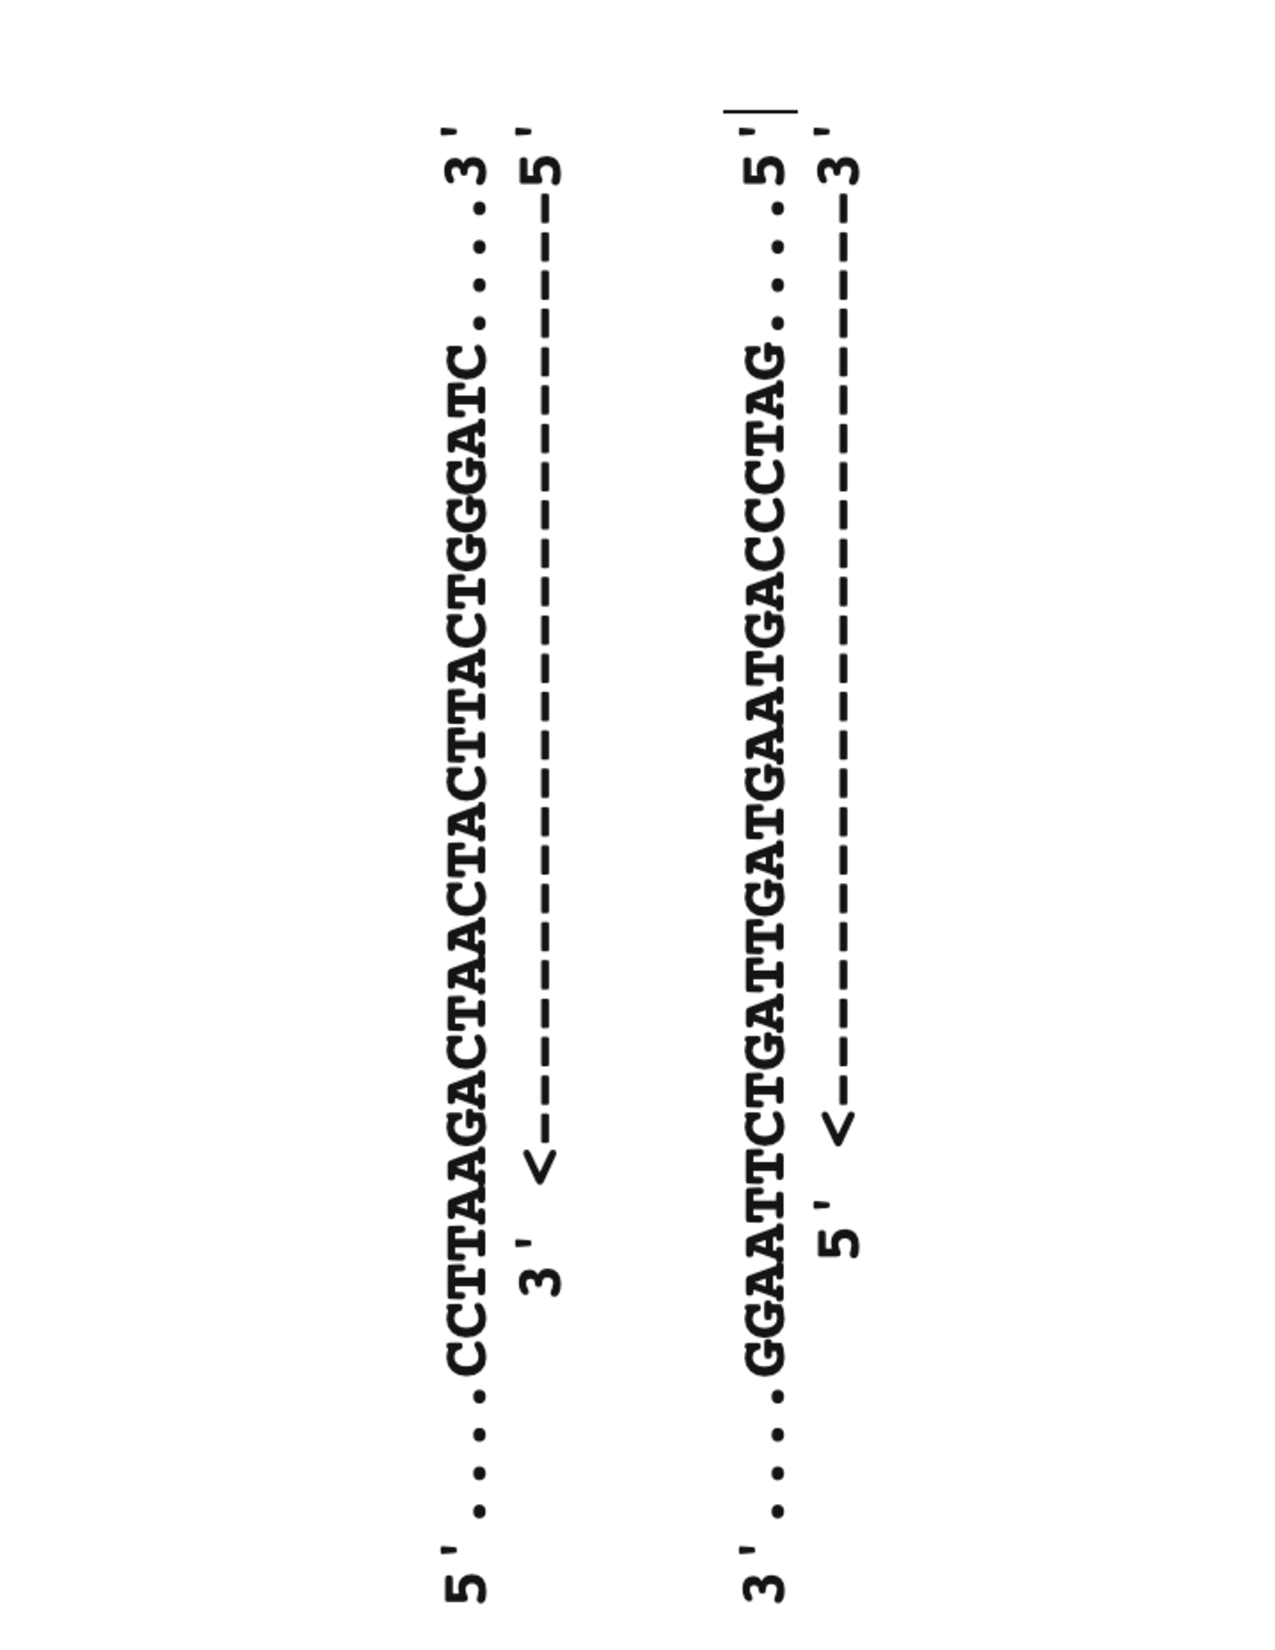
\includegraphics[angle=270, scale = 0.5]{chp7-26}
\vspace{-30mm}

Now, the question tells you that the polymerase moves from right to left. I added a crappy arrow up there to demonstrate. On the top strand, the polymerase is adding nucleotides starting with the 5' end, moving towards 3'. This is your leading strand because nucleotides can only be added when the DNA polymerase catalyzes a reaction with the 3'-OH. That is, nucleotides can only be added to the 3' end. (Imagine each nucleotide like [5'-3'][5'-3'][5'-3'][5'-3'], so that if the front is 5' it has a 3' "butt".)

Take a look at the bottom strand. As you can see, DNA polymerase would have to add from the 3' end to the 5' end, but that's not possible! The 3' starting point has a 5' butt (it is [3'-5'][3'-5'][3'-5'], in reverse orientation as above), and nucleotides cannot be added to the 5' butt. So, the bottom is the template sequence for the Okazaki fragments, i.e., the lagging strand. 

Once you know that the bottom is the template sequence, you just need to copy the opposite strand (the top one) to get the actual sequence of the Okazaki fragment:\\

5' ....CCTTAAGACTAACTACTTACTGGGATC....3'

\section{Chapter 5}

In the context of mutations in the lac operon, cis and trans refer to the effects of the mutation --- does the mutation only affect the genes of that particular chromosome (cis), or the genes of both chromosomes (trans)? 

For questions relating to linkage phase, cis and trans refer to the configuration of the dominant and recessive alleles. If the dominant alleles are on the same chromosome (eg, AB/ab), that would be cis; if they are on opposite chromosomes (eg, Ab/aB) they are in trans. 

For part c, think of those mutants as diploids (that’s what they mean by heterokaryon). So, for 1,3 and 2,4 mutants: one ``chromosome" is 1-, 2+, 3-, 4+, 5+, and the other is 1+, 2-, 3+, 4-, 5+. Notice how this organism still has one wildtype copy of each allele! Therefore, it would still grow when plated on minimal media. However, for something like 1,3 and 3,4, it wouldn’t, because it has no functional copy of the “3” allele.\\ 

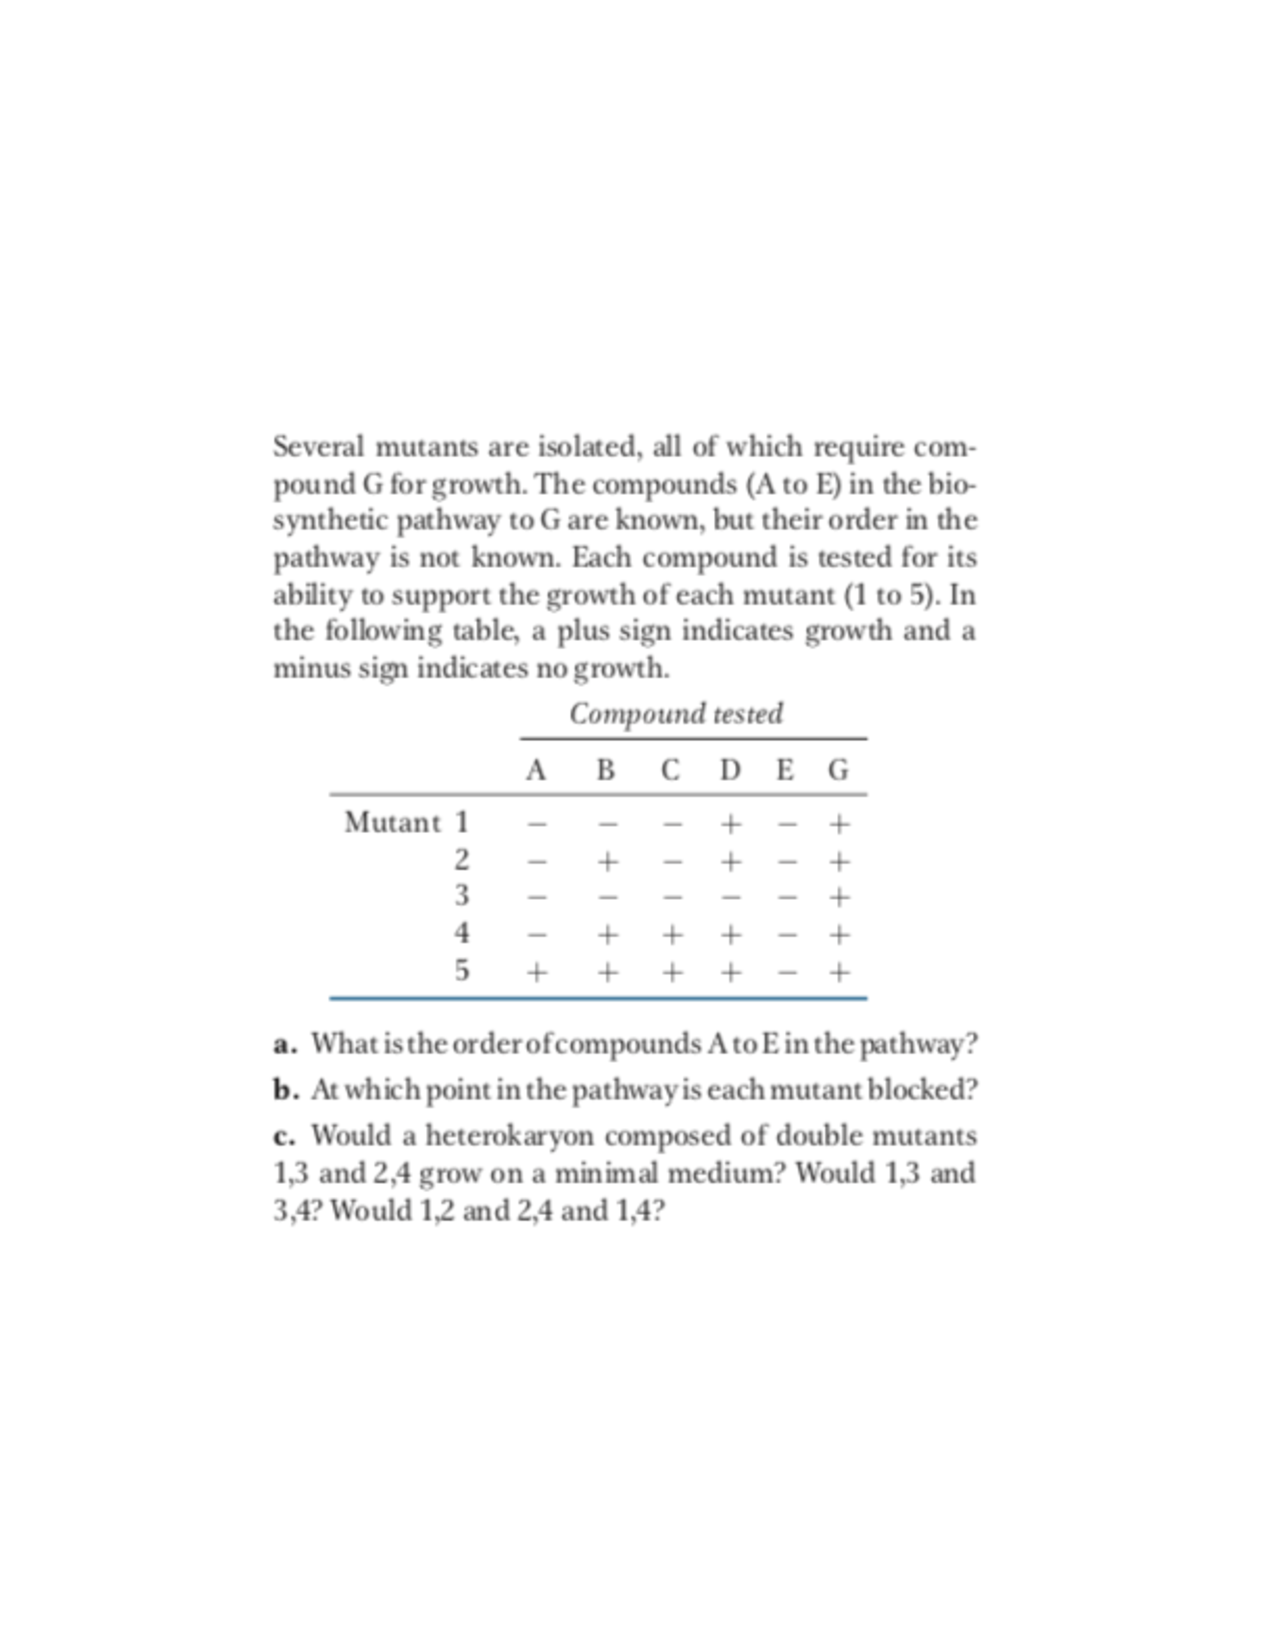
\includegraphics[width=8cm, height=10cm]{heterokaryon}


\section{Translation}
Oops! I did it again. I played with your hearts. Got lost in the game. Anyway, I didn't say the right stuff about the TATA box and the -35 and -10 consensus sequence. These are both promoters regions, just as Khalid said.

In eukaryotes --- upstream of the transcription start site, there is a sequence called the TATA box. This sequence is recognized by the TATA-binding protein (TBP), which is part of a complex that attracts other generalized transcription factors (GTFs). These transcription factors attract the RNA polymerase II to the appropriate start site. Thus, it is one type of promoter sequence found in many eukaroytes. 

In prokaryotes --- upstream of the transcription start site, there is a promoter consensus sequence (the -10 and -35 consensus sequence is found in \textit{E. coli}). This sequence of nucleotides binds to the sigma factor of the RNA polymerase holoenzyme, ensuring that it binds in the appropriate way for transcription to begin. Take a look at page 300 in your book for more information on this.


\section{Mendelian stuff}
For the second problem, remember that the wild-type (wt) organism is NOT a complementation group, it's simply there as a control. (Wild-type organisms do not have any mutations, so they can't be a complementation group.)

For the last problem, I saw a few common issues:

1. If the question asks you to report phenotypic ratios or proportions, don't just put one number! Many people wrote, for example, ``6" -- but ``6" isn't really anything on its own. Remember ``6" is simply how many you counted on a Punnett square, but that isn't the actual number of offspring. It's telling you the expected proportions of each genotype among the offspring. (Put another way, it's the probability of seeing a particular genotype each time the parents produce offspring.) So to get full credit on a test or quiz, you'll need to write ``$\frac{6}{8}$", or even better, ``$\frac{3}{4}$", or equally better, ``75\%".

2. When reporting proportions of offspring for sex-linked traits, be careful to note whether the question asks you to report male and female phenotypes together or separately. In this question, you were asked to report them separately, so you don't have $\frac{5}{16}$ mutant males -- 16 is the total number of individuals, not the total number of males! A 16-box Punnet square is going to be split equally between females and males, so to report proportions of males only, you'll need to make it out of 8. In this case, the correct answer was $\frac{5}{8}$.

\end{document}